\documentclass[11pt, a4paper]{article}

\usepackage[top = 1 in, bottom = 1 in, left = 1 in, right = 1 in]{geometry}

\usepackage{amsmath}
\allowdisplaybreaks[1]
\usepackage{amssymb, amsfonts}
\usepackage{enumerate}
\usepackage{multirow}
\usepackage{hhline}
\usepackage{array}
\usepackage{longtable}
\usepackage{graphicx}
\usepackage{tabularray}
\usepackage{undertilde}
\usepackage{dingbat}
\usepackage{fontawesome5}
\usepackage[colorlinks=true, linkcolor=blue, urlcolor=red]{hyperref}
\usepackage{tasks}
\usepackage{bbding}
\usepackage{twemojis}
% how to use bull's eye ----- \scalebox{2.0}{\twemoji{bullseye}}
\usepackage{customdice}
% how to put dice face ------ \dice{2}

\title{Principal Component Analysis}
\author{Ananda Biswas}
\date{}


\newcommand{\colvec}[2]{\begin{bmatrix} #1 \\ #2 \end{bmatrix}}


\begin{document}

\maketitle

\tableofcontents

\newpage

\section{Warming up with Linear Algebra}

\subsection{Eigenvalues and Eigenvectors}

\leftpointright \hspace{0.3cm} What happens when a matrix hits a vector? \\

\flushleft{\smallpencil} \hspace{0.2cm} The vector gets strayed from its path and becomes a new vector. The vector may also get scaled (elongated or shortened) in the process.

\begin{figure}[!htbp]

\centering

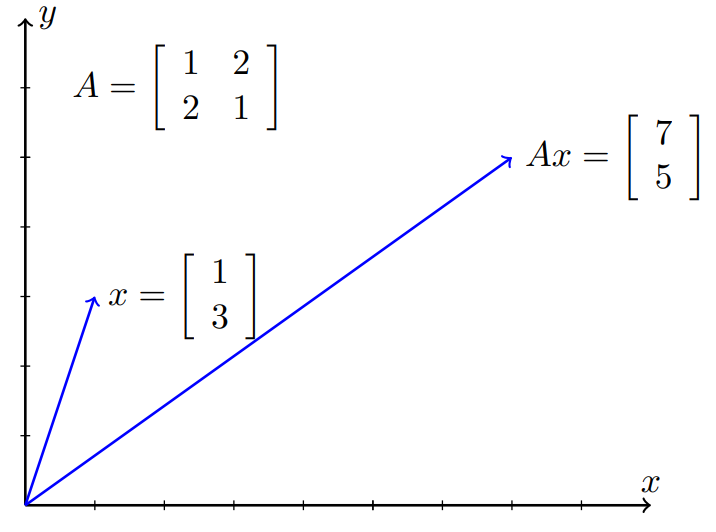
\includegraphics[scale=0.5]{image_1.png}

\end{figure}

For a given square matrix $A$, there exists special vectors which refuse to stray from their path. These vectors are called eigenvectors.

\begin{figure}[!htbp]

\centering

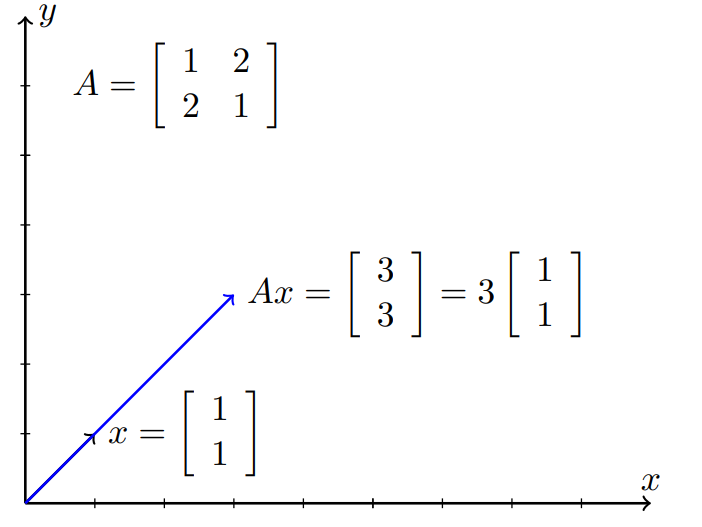
\includegraphics[scale=0.5]{image_2.png}

\end{figure}

In brief, matrix multiplications are linear transformations. Specially for square matrices, after multiplication, there stands few vectors whose respective spans remain unchanged. These vectors themselves are the eigenvectors of the matrix and the relative change in magnitude are the corresponding eigenvalues. It is also justified by the equation $A \utilde{x} = \lambda \utilde{x}$ \textit{i.e.} multiplying $\utilde{x}$ by $A$ is same as multiplying it by a constant $\lambda$. \\

\vspace{0.3cm}

\leftpointright \hspace{0.3cm} \textbf{Definition : } Let $\lambda_1, \lambda_2, \ldots, \lambda_n$ be $n$ eigenvalues of an $n \times n$ matrix $A$. $\lambda_1$ is called the \textbf{dominant eigenvalue} of $A$ if $$|\lambda_1| \geq |\lambda_i| \,\,\, \forall i = 2, 3, \ldots, n.$$

\leftpointright \hspace{0.3cm} \textbf{Definition : } A matrix $M$ is called a \textbf{column stochastic matrix} if all the entries are positive and the sum of the elements in each column is equal to 1. \\

\hspace{1cm} There are also row stochastic matrices and doubly stochastic matrices. \\

\newpage

\leftpointright \hspace{0.3cm} \textbf{Theorem : } The largest(dominant) eigenvalue of a stochastic matrix is 1. \\

\vspace{0.3cm}

\leftpointright \hspace{0.3cm}  \textbf{Theorem : } If $A$ is a $n \times n$ square matrix with a dominant eigenvalue, then the sequence of vectors given by $Av_0, A^2v_0, \ldots , A^nv_0, \ldots$ approaches a multiple of the dominant eigenvector of $A$.

\vspace{0.3cm}

\leftpointright \hspace{0.3cm}  \textbf{Theorem : } If $A$ is a square symmetric $n \times n$ matrix, then the solution to the following optimization problem is given by the eigenvector corresponding to the largest eigenvalue of $A$.

\[
\max_{\utilde{x}} \ \utilde{x}^T A \utilde{x} 
\]
\[
\text{s.t. } \|\utilde{x}\| = 1, \ \utilde{x} \in \mathbb{R}^n
\]

and the solution to

\[
\min_{\utilde{x}} \ \utilde{x}^T A \utilde{x} 
\]
\[
\text{s.t. } \|\utilde{x}\| = 1, \ \utilde{x} \in \mathbb{R}^n
\]

is given by the eigenvector corresponding to the smallest eigenvalue of $A$. \\

\vspace{0.3cm}

\underline{\textbf{proof}} : This is a constrained optimization problem that can be solved using Lagrange Multipliers:

\[
L = \utilde{x}^T A \utilde{x} - \lambda (\utilde{x}^T \utilde{x} - 1)
\]

\[
\frac{\partial L}{\partial \utilde{x}} = 2 A \utilde{x} - \lambda (2\utilde{x}) = 0 \Rightarrow A \utilde{x} = \lambda \utilde{x}
\]\\[1.5em]

Hence $\utilde{x}$ must be an eigenvector of $A$ with eigenvalue $\lambda$. \\[1.5em]

Multiplying by $\utilde{x}^T$:

\[
\utilde{x}^T A \utilde{x} = \lambda \utilde{x}^T \utilde{x} = \lambda \ (\text{since } \utilde{x}^T \utilde{x} = 1)
\]

Therefore, the critical points of this constrained problem are the eigenvalues of $A$. \\[1.5em]

The maximum value is the largest eigenvalue, while the minimum value is the smallest eigenvalue.

\newpage

\subsection{More Linear Algebra}

\leftpointright \hspace{0.3cm} \textbf{Definition : } A set of $n$ vectors $v_1, v_2, \ldots , v_n$ is called \textbf{linearly independent} 
if and only if no vector in the set can be expressed as a linear combination of the remaining $n - 1$ vectors. \\

\vspace{0.3cm}

\leftpointright \hspace{0.3cm} \textbf{Definition : } A set of vectors $\in \mathbb{R}^n$ is called a \textbf{basis}, if they are linearly independent and every vector $\in \mathbb{R}^n$ can be expressed as a linear combination of these vectors. \\

\vspace{0.3cm}

\leftpointright \hspace{0.3cm} Consider the space $\mathbb{R}^2$ and two vectors $\utilde{x} =  \begin{bmatrix} 1 \\ 0 \end{bmatrix} $ and $\utilde{y} =  \begin{bmatrix} 0 \\ 1 \end{bmatrix} $.

\begin{figure}[!htbp]

\centering

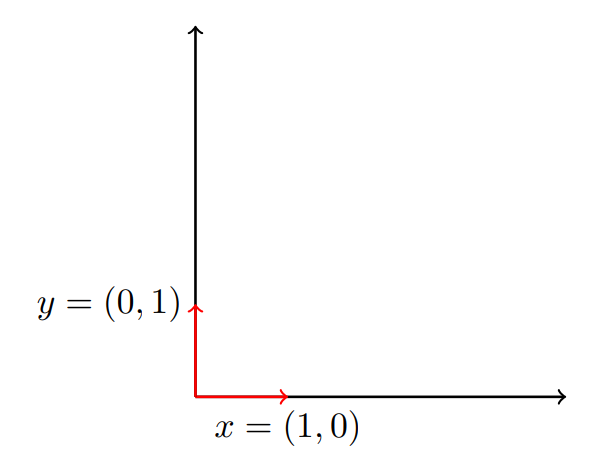
\includegraphics[scale=0.5]{image_3.png}

\end{figure}

Any vector $\begin{bmatrix} a \\ b \end{bmatrix}$ can be expressed as a linear combination of these two vectors \textit{i.e.}

\begin{gather*}
\begin{bmatrix} a \\ b \end{bmatrix}
= 
a \begin{bmatrix} 1 \\ 0 \end{bmatrix}
+
b \begin{bmatrix} 0 \\ 1 \end{bmatrix}.
\end{gather*}

And indeed we are used to representing all vectors in $\mathbb{R}^2$ as a linear combination of these two vectors. But there is nothing sacrosanct about this particular choice of $\utilde{x}$ and $\utilde{y}$. 
We could have chosen any 2 linearly independent vectors in $\mathbb{R}^2$ as the basis vectors. \\

\vspace{0.3cm}

For example, consider the linearly independent vectors, $\colvec{2}{3}$ and $\colvec{5}{7}$. See how any vector $\colvec{a}{b} \in \mathbb{R}^2$ can be expressed as a linear combination of these two vectors.

\begin{gather*}
\colvec{a}{b} = x_1 \colvec{2}{3} + x_2 \colvec{5}{7}.
\end{gather*}

We can find $x_1$ and $x_2$ by solving a system of equations

\begin{align*}
a &= 2x_1 + 5x_2 \\
b &= 3x_1 + 7x_2
\end{align*}

\newpage

In general, given a set of linearly independent vectors $\utilde{u_1}, \utilde{u_2}, \ldots, \utilde{u_n} \in \mathbb{R}^n$, we can express any vector $\utilde{z} \in \mathbb{R}^n$ as a linear combination of these
vectors.

\begin{figure}[!htbp]

\centering

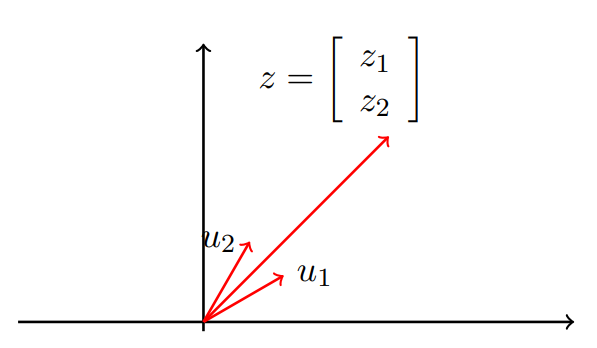
\includegraphics[scale=0.5]{image_4.png}

\end{figure}


\begin{align*}
\utilde{z} &= \alpha_1 \utilde{u_1} + \alpha_2 \utilde{u_2} + \cdots + \alpha_n \utilde{u_n} \\[1.5em]
\Rightarrow \begin{bmatrix}
z_1 \\
z_2 \\
\vdots \\
z_n
\end{bmatrix}
&=
\alpha_1
\begin{bmatrix}
u_{11} \\
u_{12} \\
\vdots \\
u_{1n}
\end{bmatrix}
+
\alpha_2
\begin{bmatrix}
u_{21} \\
u_{22} \\
\vdots \\
u_{2n}
\end{bmatrix}
+ \cdots +
\alpha_n
\begin{bmatrix}
u_{n1} \\
u_{n2} \\
\vdots \\
u_{nn}
\end{bmatrix}
\\[1.5em]
\Rightarrow \begin{bmatrix}
z_1 \\
z_2 \\
\vdots \\
z_n
\end{bmatrix}
&=
\begin{bmatrix}
u_{11} & u_{21} & \cdots & u_{n1} \\
u_{12} & u_{22} & \cdots & u_{n2} \\
\vdots & \vdots & \ddots & \vdots \\
u_{1n} & u_{2n} & \cdots & u_{nn}
\end{bmatrix}
\begin{bmatrix}
\alpha_1 \\
\alpha_2 \\
\vdots \\
\alpha_n
\end{bmatrix}
\end{align*}

We can now find the $\alpha_i$'s using Gaussian Elimination (Time Complexity: $O(n^3))$. \\

\vspace{0.3cm}

\leftpointright \hspace{0.3cm} Now let us see if we have orthonormal basis.

\begin{figure}[!htbp]

\centering

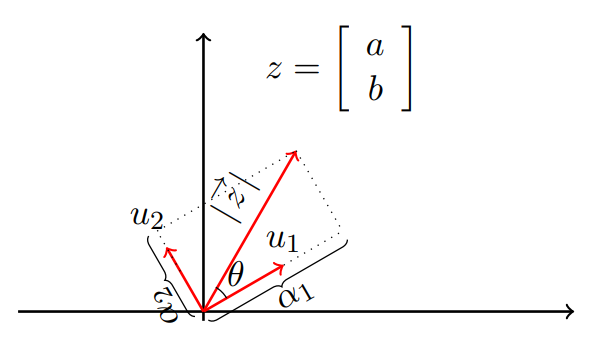
\includegraphics[scale=0.5]{image_5.png}

\end{figure}

Then $\utilde{u_i}^T \utilde{u_j} = 0 \ \forall i \neq j$ and $\utilde{u_i}^T \utilde{u_i} = \| \utilde{u_i} \|^2 = 1$. \\[0.3cm]

Again we have:

\begin{align*}
\utilde{z} &= \alpha_1 \utilde{u_1} + \alpha_2 \utilde{u_2} + \cdots + \alpha_n \utilde{u_n} \\ 
\Rightarrow \utilde{u_1}^T \utilde{z} &= \alpha_1 \utilde{u_1}^T \utilde{u_1} + \cdots + \alpha_n \utilde{u_1}^T \utilde{u_n} \\ &= \alpha_1
\end{align*}

We can directly find each \( \alpha_i \) using a dot product between \( z \) and \( \utilde{u_i} \)
(time complexity \( O(N) \)). \\[0.3cm]

The total complexity will be $O(N^2)$.

\newpage

Also from figure, $\alpha_1 = |\utilde{z}| \cos \theta = |\utilde{z}| \cdot \dfrac{\utilde{z}^T \utilde{u_1}}{|\utilde{z}| |\utilde{u_1}|} = \utilde{z}^T \utilde{u_1}$. \\

\vspace{0.3cm}

Similarly, $\alpha_2 = \utilde{z}^T \utilde{u_2}$. \\

\vspace{0.3cm}

So, \textbf{an orthonormal basis is the most convenient basis that one can hope for}. \\

\vspace{0.3cm}

\leftpointright \hspace{0.3cm} Turns out that the eigenvectors can form a basis. In fact, the eigenvectors of a square symmetric matrix are orthogonal and thus they form a very convenient basis. But why would we want to use the eigenvectors as a basis instead of the more natural co-ordinate axes? We will find the answer in PCA. \\

\subsection{Eigenvalue Decomposition}

Let $\utilde{u_1}, \utilde{u_2}, \ldots, \utilde{u_n}$ be the eigenvectors of a square matrix $A$ and let $\lambda_1, \lambda_2, \ldots, \lambda_n$ be the corresponding eigenvalues. \\[1.5em]

Consider a matrix $U$ whose columns are $\utilde{u_1}, \utilde{u_2}, \ldots, \utilde{u_n}$. \\[1.5em]

Now

\begin{align*}
AU &= A \begin{bmatrix}
\uparrow & \uparrow & & \uparrow \\
\utilde{u_1} & \utilde{u_2} & \cdots & \utilde{u_n} \\
\downarrow & \downarrow & & \downarrow
\end{bmatrix} \\[1.5em]
&= \begin{bmatrix}
\uparrow & \uparrow & & \uparrow \\
A\utilde{u_1} & A\utilde{u_2} & \cdots & A\utilde{u_n} \\
\downarrow & \downarrow & & \downarrow
\end{bmatrix} \\[1.5em]
&= \begin{bmatrix}
\uparrow & \uparrow & & \uparrow \\
\lambda_1 \utilde{u_1} & \lambda_2 \utilde{u_2} & \cdots & \lambda_n \utilde{u_n} \\
\downarrow & \downarrow & & \downarrow
\end{bmatrix} \\[1.5em]
&= \begin{bmatrix}
\uparrow & \uparrow & & \uparrow \\
\utilde{u_1} & \utilde{u_2} & \cdots & \utilde{u_n} \\
\downarrow & \downarrow & & \downarrow
\end{bmatrix} \cdot
\begin{bmatrix}
\lambda_1 & 0 & \cdots & 0 \\
0 & \lambda_2 & \cdots & \vdots \\
\vdots & \vdots & \ddots & 0 \\
0 & \cdots & 0 & \lambda_n
\end{bmatrix} \\[1.5em]
&= U \Lambda
\end{align*}

where $\Lambda$ is a diagonal matrix whose diagonal elements are the eigenvalues of $A$. \\

\vspace{0.3cm}

$\therefore AU = U\Lambda$. \\

\vspace{0.3cm}

Now, if the columns of $U$ are linearly independent \textit{i.e.} if $A$ has $n$ linearly independent eigenvectors \textit{i.e.} if $A$ has $n$ distinct eigenvalues, then $U^{-1}$ exists and we can write

\begin{align*}
A &= U \Lambda U^{-1} \hspace{0.2cm} \text{[eigenvalue decomposition]} \\
U^{-1} A U &= \Lambda \hspace{1.2cm} \text{[diagonalization of } A]
\end{align*}

\newpage

If $A$ is symmetric then the situation is even more convenient. The eigenvectors are orthogonal. Further let's assume, that the eigenvectors have been normalized. $\left[ \utilde{u_i}^T \utilde{u_i} = 1 \right]$

Then,
\[
Q = U^T U =
\begin{bmatrix}
\leftarrow u_1 \rightarrow \\
\leftarrow u_2 \rightarrow \\
\vdots \\
\leftarrow u_n \rightarrow
\end{bmatrix}
\begin{bmatrix}
\uparrow & \uparrow & & \uparrow \\
u_1 & u_2 & \cdots & u_n \\
\downarrow & \downarrow & & \downarrow
\end{bmatrix}
\]

Each entry of the matrix, $Q_{ij}$ is given by $\utilde{u_i}^T \utilde{u_i}$

\[
Q_{ij} = \utilde{u_i}^T \utilde{u_i} =
\begin{cases}
0 & \text{if } i \neq j \\
1 & \text{if } i = j
\end{cases}
\]

\[
\therefore U^T U = \mathbb{I} \ \text{(the identity matrix)}
\]

So $U^T$ is the inverse of $U$ (very convenient to calculate).

\subsection{The story so far \ldots}

\begin{enumerate}[$\bullet$]

\item The eigenvectors corresponding to different eigenvalues are linearly independent.

\item The eigenvectors of a square symmetric matrix are orthogonal.

\item The eigenvectors of a square symmetric matrix can thus form a convenient basis.

\end{enumerate}

We will put all these to use.



\section{Principal Component Analysis}

The objective of Principal Component Analysis is to make a new representation of the data. We are also compressing the data and we want the compression to be as loss-less as possible. It is a \underline{feature extraction} technique.

\subsection{Interpretation 1}

$\bullet$ Consider the following data.

\begin{figure}[!htbp]

\centering

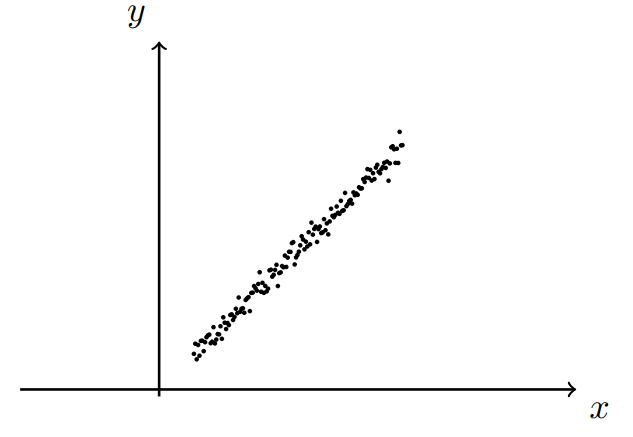
\includegraphics[scale=0.5]{image_7.png}

\end{figure}

Each point (vector) here is represented using a linear combination of the $x$ and $y$ axes (\textit{i.e.} using the point’s $x$ and $y$ co-ordinates). In other words we are using $x-$axis and $y-$axis as the basis. What if we choose a different basis? \\

\hspace{0.3cm}

\begin{figure}[!htbp]

\centering

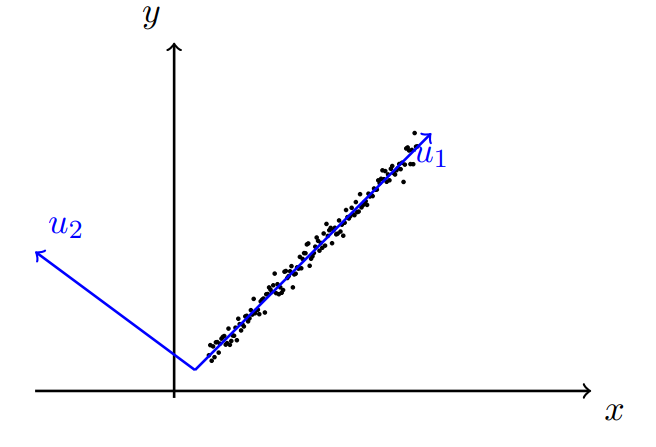
\includegraphics[scale=0.5]{image_8.png}

\end{figure}

For example, what if we use $\utilde{u_1}$ and $\utilde{u_2}$ as a basis instead of $x-$axis and $y-$axis. We observe that all the points have a
very small component in the direction of $\utilde{u_2}$ (almost noise). It seems that the same data which was originally in $\mathbb{R}^2 (x, y)$ can now be represented in $\mathbb{R}^1(u_1)$ by making a smarter choice for the basis. \\

\hspace{0.3cm}

But why not care about $\utilde{u_2}$ ? Because the variance in the data in this direction is very small (all data points have almost the same value in the $\utilde{u_2}$ direction).

\begin{figure}[!htbp]

\centering

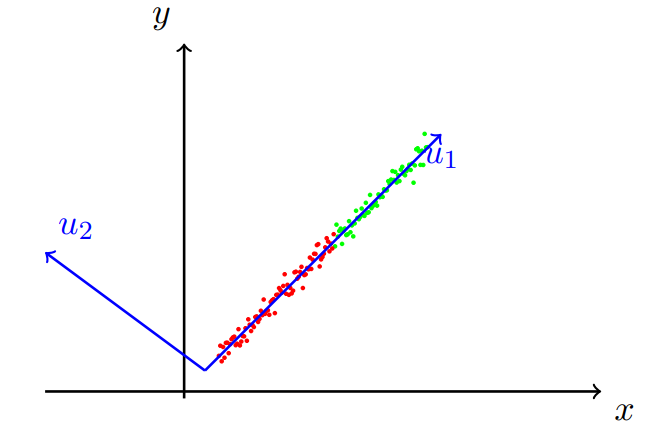
\includegraphics[scale=0.5]{image_9.png}

\end{figure}

If we were to build a classifier on top of this data then $\utilde{u_2}$ would not contribute to the classifier as the points are not distinguishable along this direction. \\

\hspace{0.3cm}

In general, we are interested in representing the data using fewer dimensions such that the data has high variance along these dimensions. But this is not all what we desire. \\[1.5em]

$\bullet$ Consider the following data.

\begin{figure}[!htbp]

\centering

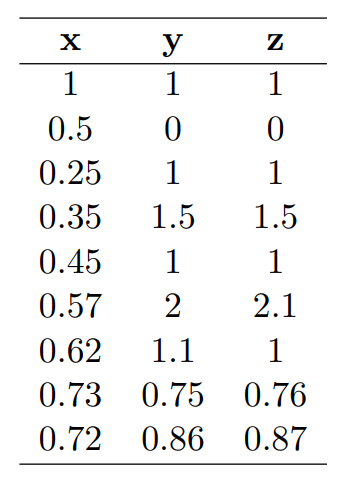
\includegraphics[scale=0.5]{image_10.png}

\end{figure}

Notice that $y$ and $z$ are highly correlated. So $z$ adds no new information beyond what is already contained in $y$. In other words, $z$ is redundant as it is largely linearly dependent on $y$. \\

\hspace{0.3cm}

\scalebox{1.5}{\twemoji{bullseye}} So in general, in PCA, we are interested in representing the data using \underline{fewer dimensions} (not in the sense of throwing away some dimensions, it is going to be a new set of dimensions; chopping off dimensions  \scalebox{1.5}{\twemoji{cross mark}}, transforming the data \scalebox{1.5}{\twemoji{check mark button}}) such that

\begin{enumerate}[(i)]

\item The data has high variance along these dimensions;

\item The dimensions are linearly independent (uncorrelated); even better if they are orthogonal because that will be a very convenient basis. \\

\end{enumerate}


\vspace{0.3cm}

$\bullet$ Now let $\utilde{p_1}, \utilde{p_2}, \ldots , \utilde{p_n}$ be a set of such $n$ linearly independent orthonormal vectors. Let $P$ be a $n \times n$ matrix such that $\utilde{p_1}, \utilde{p_2}, \ldots , \utilde{p_n}$ are the columns of $P$. \\

\vspace{0.3cm}

Let $\utilde{x_1}, \utilde{x_2}, \ldots , \utilde{x_m} \in \mathbb{R}^n$ be $m$ data points and let $X$ be a matrix such that $\utilde{x_1}, \utilde{x_2}, \ldots , \utilde{x_m}$ are the rows of this matrix. Further let us assume that the data is $0-$mean and unit variance. \\

\vspace{0.3cm}

We want to represent each $\utilde{x_i}$ using this new basis $P$ as follows.

$$\utilde{x_i} = \alpha_{i1} \utilde{p_1} + \alpha_{i2} \utilde{p_2} + \alpha_{i3} \utilde{p_3} + \ldots + \alpha_{in} \utilde{p_n}.$$

For an orthonormal basis we know that we can find these $\alpha_{ij}'$s using

\[
\alpha_{ij} = \utilde{x_i}^T \utilde{p_j} = 
\left[
\leftarrow \; \utilde{x_i} \; \rightarrow
\right]
\begin{bmatrix}
\uparrow \\
\utilde{p_j} \\
\downarrow
\end{bmatrix}
\]

In general, the transformed data $\utilde{\hat{x}_i}$ is given by

\[
\utilde{\hat{x}_i} = 
\left[ \leftarrow \; \utilde{x_i} \; \rightarrow \right]
\begin{bmatrix}
\uparrow & & \uparrow \\
\utilde{p_1} & \cdots & \utilde{p_n} \\
\downarrow & & \downarrow
\end{bmatrix}
= \utilde{x_i}^T P 
= \left( \alpha_{i1}, \alpha_{i2}, \ldots, \alpha_{in} \right)_{1 \times n}
\]

and

\[
\hat{X} = X P
\qquad (\hat{X} \text{ is the matrix of transformed points})
\]


$\blacksquare$ \textbf{\underline{Theorem}} :
If $X$ is a matrix such that its columns have zero mean and if $\hat{X} = X P$ then the columns of $\hat{X}$ will also have zero mean.

$\blacktriangleright$ \textbf{Proof :}
For any matrix $A$, $\mathbf{1}^T A$ gives us a row vector with the $i^{th}$ element containing the sum of the $i^{th}$ column of $A$. (This is easy to see using the row-column picture of matrix multiplication). \\
Consider
\[
\mathbf{1}^T \hat{X} = \mathbf{1}^T X P = \left(\mathbf{1}^T X\right) P
\]
But $\mathbf{1}^T X$ is the row vector containing the sums of the columns of $X$. Thus $\mathbf{1}^T X = \utilde{0}$. Therefore, $\mathbf{1}^T \hat{X} = \utilde{0}$. \\
Hence the transformed matrix also has columns with sum = 0.

\vspace{1em}

$\blacksquare$ \textbf{\underline{Theorem}} :
$X^T X$ is a symmetric matrix.

$\blacktriangleright$ \textbf{Proof :}
We can write
\[
\left( X^T X \right)^T = X^T \left( X^T \right)^T = X^T X
\]


$\blacksquare$ \textbf{\underline{Result}} :
If $X$ is a matrix whose columns are zero mean then $\Sigma = \dfrac{1}{m} X^T X$ is the covariance matrix. In other words, each entry $\sigma_{ij}$ stores the covariance between columns $i$ and $j$ of $X$.

\vspace{1em}

$\blacktriangleright$ \textbf{Explanation} :
Let $\Sigma$ be the covariance matrix of $X$. Let $\mu_i, \mu_j$ denote the means of the $i^{th}$ and $j^{th}$ column of $X$ respectively. Then by definition of covariance, we can write:

\begin{align*}
\sigma_{ij} &= \dfrac{1}{m} \sum\limits_{k=1}^{m} (X_{ki} - \mu_i)(X_{kj} - \mu_j) \\[0.5em]
&= \dfrac{1}{m} \sum\limits_{k=1}^{m} X_{ki} X_{kj} \hspace{1cm} [\because \mu_i = \mu_j = 0] \\[0.5em]
&= \dfrac{1}{m} X_i^T X_j \\[0.5em]
&= \dfrac{1}{m} \left( X^T X \right)_{ij}
\end{align*}

$\bullet$ We have $\hat{X} = X P$. Using the previous theorems \& result, we get $\dfrac{1}{m} \hat{X}^T \hat{X}$ is the covariance matrix of the transformed data. We can write:
    \[
    \dfrac{1}{m} \hat{X}^T \hat{X} = \dfrac{1}{m} (X P)^T X P = \dfrac{1}{m} P^T X^T X P = P^T \left(\dfrac{1}{m} X^T X\right) P = P^T \Sigma P
    \]
    
We know each cell $i, j$ of the covariance matrix $\dfrac{1}{m} \hat{X}^T \hat{X}$ stores the covariance between columns $i$ and $j$ of $\hat{X}$. Ideally, we want
\begin{align*}
\left(\dfrac{1}{m} \hat{X}^T \hat{X}\right)_{ij} &= 0 \qquad \text{if } i \neq j \ (\text{covariance = 0}) \\
\left(\dfrac{1}{m} \hat{X}^T \hat{X}\right)_{ij} &\neq 0 \qquad \text{if } i = j \ (\text{variance } \neq 0)
\end{align*}
    
In other words, we want
\[
\dfrac{1}{m} \hat{X}^T \hat{X} = P^T \Sigma P = D. \hspace{1cm} \text{[ where D is a diagonal matrix ]}
\]

$\bullet$ We want $P^T \Sigma P = D$ where $\Sigma$ is a square matrix and $P$ is an orthogonal matrix. \\

\vspace{0.3cm}

Now the question is which orthogonal matrix satisfies the following condition $P^T \Sigma P = D $ . \\

\vspace{0.3cm}

In other words, which orthogonal matrix $P$ diagonalizes $\Sigma$? Answer is a matrix $P$ whose columns are the eigenvectors of $\Sigma = \dfrac{1}{m} X^T X$ [by Eigenvalue Decomposition]. \\

\vspace{0.3cm}

Thus, the new basis $P$ used to transform $X$ is the basis consisting of the eigenvectors of $\dfrac{1}{m} X^T X$. \\

\vspace{0.3cm}

$\bullet$ Why is this a good basis? Because the eigenvectors of $\dfrac{1}{m}X^T X$ are linearly independent and because the eigenvectors of $\dfrac{1}{m}X^T X$ are orthogonal. \\

\vspace{0.3cm}

$\bullet$ This method is called Principal Component Analysis for transforming the data to a new basis where the dimensions are non-redundant (low covariance) \& not noisy (high variance). \\

\vspace{0.3cm}

In practice, we select only the top-$k$ dimensions along which the variance is high (this will become more clear when we look at an alternate interpretation of PCA).

\newpage

\subsection{Interpretation 2}

Given $n$ orthogonal linearly independent vectors $\utilde{p_1}, \utilde{p_2}, \ldots, \utilde{p_n}$, we can represent $\utilde{x_i}$ \underline{exactly} (exactly only when we use all $\utilde{p_i}$'s, it will be approximate when we discard some of $\utilde{p_i}$'s) as a linear combination of these vectors as follows.
\[
\utilde{x_i} = \sum_{j=1}^{n} \alpha_{ij} \utilde{p_j} \hspace{1cm}  \text{[we know how to estimate $\alpha_{ij}$'s but we will come back to that later]}
\]

But we are interested only in the top-$k$ dimensions (we want to get rid of noisy \& redundant dimensions)
\[
\utilde{\hat{x}_i} = \sum_{j=1}^{k} \alpha_{ij} \utilde{p_j}
\]

So we want to select $p_i$'s such that we minimise the \underline{reconstructed error} :
\[
e = \sum_{i=1}^{m} (\utilde{x_i} - \utilde{\hat{x}_i})^T (\utilde{x_i} - \utilde{\hat{x}_i})
\]

Now, 
\begin{align*}
e &= \sum_{i=1}^{m} (\utilde{x_i} - \utilde{\hat{x}_i})^T (\utilde{x_i} - \utilde{\hat{x}_i}) \\[0.75em]
&= \sum_{i=1}^m \left( \sum_{j=1}^n \alpha_{ij} \utilde{p_j} - \sum_{j=1}^k \alpha_{ij} \utilde{p_j} \right)^T \left( \sum_{j=1}^n \alpha_{ij} \utilde{p_j} - \sum_{j=1}^k \alpha_{ij} \utilde{p_j} \right) \\[0.75em]
&= \sum_{i=1}^m \left[ \left( \sum_{j=k+1}^n \alpha_{ij} p_j \right)^T \left( \sum_{j=k+1}^n \alpha_{ij} p_j \right) \right] \\[0.75em]
&= \sum_{i=1}^m \left( \alpha_{i,k+1} \cdot \utilde{p_{k+1}} + \alpha_{i,k+2} \cdot \utilde{p_{k+2}} + \ldots + \alpha_{i,n} \cdot \utilde{p_n} \right)^T \left( \alpha_{i,k+1} \cdot \utilde{p_{k+1}} + \alpha_{i,k+2} \cdot \utilde{p_{k+2}} + \ldots + \alpha_{i,n} \cdot \utilde{p_n} \right) \\[0.75em]
&= \sum_{i=1}^m \left( \alpha_{i,k+1} \cdot \utilde{p_{k+1}}^T + \alpha_{i,k+2} \cdot \utilde{p_{k+2}}^T + \ldots + \alpha_{i,n} \cdot \utilde{p_n}^T \right) \left( \alpha_{i,k+1} \cdot \utilde{p_{k+1}} + \alpha_{i,k+2} \cdot \utilde{p_{k+2}} + \ldots + \alpha_{i,n} \cdot \utilde{p_n} \right) \\[0.75em]
&= \sum_{i=1}^m \left( \sum_{j=k+1}^n \alpha_{ij} \utilde{p_j}^T \cdot \alpha_{ij} \utilde{p_j} \right) + \sum_{i=1}^m \left( \sum_{j=k+1}^n \sum_{L=k+1, L \neq k}^n \alpha_{ij} \utilde{p_j}^T \cdot \alpha_{iL} \utilde{p_L} \right) \\[0.75em]
&= \sum_{i=1}^m \sum_{j=k+1}^n \alpha_{ij} \utilde{p_j}^T \utilde{p_j} \alpha_{ij} + \sum_{i=1}^m \sum_{j=k+1}^n \sum_{L=k+1, L \neq k}^n \alpha_{ij} \utilde{p_j}^T \utilde{p_L} \alpha_{iL} \\[0.75em]
&= \sum_{i=1}^m \sum_{j=k+1}^n \alpha_{ij}^2 \qquad 
(\because \utilde{p_j}^T \utilde{p_j} = 1, \ \utilde{p_i}^T \utilde{p_j} = 0 \,\, \forall i \neq j)  \\[0.75em]
&= \sum_{i=1}^m \sum_{j=k+1}^n \left( \utilde{x_i}^T \utilde{p_j} \right)^2 \\[0.75em] 
&= \sum_{i=1}^{m} \sum_{j=k+1}^{n} \left( \utilde{p_j}^T x_i \right) \left( x_i^T \utilde{p_j} \right) \\[0.75em]
&= \sum_{j=k+1}^{n} \utilde{p_j}^T \left( \sum_{i=1}^{m} \utilde{x_i} \utilde{x_i}^T \right) \utilde{p_j} \\[0.75em]
&= \sum_{j=k+1}^{n} \utilde{p_j}^T \, m \Sigma \, \utilde{p_j} \qquad \left[ \because \frac{1}{m} \sum_{i=1}^{m} \utilde{x_i} \utilde{x_i}^T = \frac{X^T X}{m} = \Sigma \right]
\end{align*}

So we want to minimize
\[
\min_{\utilde{p_{k+1}}, \utilde{p_{k+2}}, \ldots, \utilde{p_n}} \sum_{j=k+1}^{n} \utilde{p_j}^T m \Sigma \utilde{p_j}
\qquad \text{s.t. } \utilde{p_j}^T \utilde{p_j} = 1 \quad \forall j = k+1, k+2, \ldots, n
\]

The solution to the above problem is given by the eigenvectors corresponding to the smallest eigenvalues of $\Sigma$ (Proof : refer to theorems in Section 1). \\

\vspace{0.3cm}

Thus we select $\utilde{p_1}, \utilde{p_2}, \ldots, \utilde{p_n}$ as eigenvectors of $\Sigma$ and retain only top-$k$ eigenvectors to express the data [or discard the eigenvectors $\utilde{p_{k+1}}, \utilde{p_{k+2}}, \ldots, \utilde{p_n}$]. \\

\vspace{0.3cm}

Here the key idea was to minimize the error in reconstructing $\utilde{x_i}$ after projecting the data on to a new basis. \\

\vspace{0.3cm}

$\spadesuit$ A quick recap :

\begin{itemize}
\item The eigenvectors of a matrix with distinct eigenvalues are linearly independent.
\item The eigenvectors of a square symmetric matrix are orthogonal.
\item PCA exploits this fact by representing the data using a new basis comprising only the top-$k$ eigenvectors.
\item The $n - k$ dimensions which contribute very little to the reconstruction error are discarded. These are also the directions along which the variance is minimum (we shall establish this in yet another interpretation of PCA).
\end{itemize}


\subsection{Interpretation 3}

We started off with the following wishlist. \\

\vspace{0.3cm}

We are interested in representing the data using fewer dimensions such that
\begin{itemize}
\item the dimensions have low covariance
\item the dimensions have high variance
\end{itemize}

So far we have paid a lot of attention to the covariance. But what about variance? Have we achieved our stated goal of high variance along dimensions? To answer this question we will see yet another interpretation of PCA. \\

\vspace{0.3cm}

The \( i^{\text{th}} \) dimension of the transformed data \( \hat{X} \) is given by
\[
\utilde{\hat{X}_i} = Xp_i
\]

The variance along this dimension is given by
\begin{align*}
\dfrac{\utilde{\hat{X}_i}^T \utilde{\hat{X}_i}}{m} &= \dfrac{1}{m} \utilde{p_i}^T X^T X \utilde{p_i} \\
&= \utilde{p_i}^T \underbrace{\dfrac{1}{m} X^T X \utilde{p_i}} \\
&= \utilde{p_i}^T \underbrace{\Sigma \utilde{p_i}} \\
&= \utilde{p_i}^T \lambda_i \utilde{p_i} \qquad [\because \utilde{p_i} \text{ is an eigenvector of } \Sigma]  \\
&= \lambda_i \underbrace{\utilde{p_i}^T \utilde{p_i}}_{=1} \\
&= \lambda_i
\end{align*}

\begin{itemize}
    \item Thus the variance along the \( i^{\text{th}} \) dimension (\( i^{\text{th}} \) eigenvector of \( \Sigma \)) is given by the corresponding eigenvalue.
    \item Hence, we did the right thing by discarding the dimensions (eigenvectors) corresponding to lower eigenvalues!
\end{itemize}

$\spadesuit$ \underline{A Quick Summary} : We have seen 3 different interpretations of PCA.
\begin{itemize}
\item It ensures that the covariance between the new dimensions are minimized.
\item It picks up dimensions such that the data exhibit high variance across these dimensions.
\item It ensures that the data can be represented using less number of dimensions.
\end{itemize}


$\spadesuit$ \underline{Note} : The total variability caused by the initial feature set \textit{i.e.} $\utilde{X_1}, \utilde{X_2}, \ldots, \utilde{X_n}$ is same as the total variability caused by the transformed feature set \textit{i.e.} $\utilde{\hat{X_1}}, \utilde{\hat{X_2}}, \ldots, \utilde{\hat{X_n}}$. How ? 
\begin{align*}
\text{Total variation due to } \utilde{X_1}, \utilde{X_2}, \ldots, \utilde{X_n} &= \text{sum of the principal diagonal elements of } \Sigma \\[0.75em]
&= \text{trace }(\Sigma) \\[0.75em]
&= \text{sum of the eigenvalues of }\Sigma \\[0.75em]
&= \text{Total variation due to } \utilde{\hat{X_1}}, \utilde{\hat{X_2}}, \ldots, \utilde{\hat{X_n}}.
\end{align*}


$\spadesuit$ \underline{Terminology} : $\utilde{\hat{X_1}}$ is called the \textbf{First Principal Component}, $\utilde{\hat{X_2}}$ is called the \textbf{Second Principal Component} and so on $\ldots$ \\

\vspace{0.3cm}

$\spadesuit$ The algorithm for PCA is an \underline{Unsupervised Learning Algorithm}.
\end{document}